\documentclass[12pt]{beamer}

\mode<presentation> {
	
	
	%\usetheme{Madrid}
	%\usepackage{times}
	\renewcommand{\familydefault}{\rmdefault}
	\usetheme{CambridgeUS}
	\usepackage[latin1]{inputenc}
	\usefonttheme{professionalfonts}
	\usepackage{times}
	\usepackage{tikz}
	\usepackage{amsmath}
	\usepackage{verbatim}
	\usepackage{enumerate}
	\usepackage{setspace}
	\usetikzlibrary{arrows,shapes}
	\usepackage{amsmath}
	\usepackage{eurosym}
	\usepackage{framed}
	\usepackage{extarrows}

}

\usepackage{graphicx}
\usepackage{booktabs}
\usepackage{url}

%----------------------------------------------------------------------------------------
%	TITLE PAGE
%----------------------------------------------------------------------------------------


\title{PP plot against Generalized Extreme Value Distribution}

\author[Group ID: No.12]{Project ID: No.13} % Your name
\institute[]{
	\textsl{Group ID: No.12}
}
\date[July 18$^{th}, 2016$]{} % Date, can be changed to a custom date







\begin{document}
	
\begin{frame}
	\titlepage
\end{frame}


\begin{frame}
	\frametitle{Outline}
	\tableofcontents
\end{frame}

\section{Introduction}

\begin{frame}
	\frametitle{Introduction}
	\quad  PP plot of tail values of daily log-returns of portfolio against Generalized Extreme Value Distribution with a global parameter $\gamma$ estimated with the block maxima method.
\end{frame}




\section{Data source}
\begin{frame}
	\frametitle{Data source}
    \begin{itemize}
	  \item The data is the daily closing stock prices of 3 DAX companies, namely \textbf{Bayer}, \textbf{BMW} and \textbf{Siemens}, from 2000-01-01 to 2016-07-11. For each company, there are 4281 observations.\\
      \item 3 stocks (\textbf{Bayer}, \textbf{BMW} and \textbf{Siemens}) form an equally-weighted portfolio from the initial dataset.
    \end{itemize}
    \quad Remark: All data comes from the YAHOO FINANCE website.
\end{frame}


\section{Procedure}
\begin{frame}
	\frametitle{Procedure}
		1.Construct a portfolio: $p=Bayer+Bmw+Siemens$
\end{frame}


\section{Procedure}

\begin{frame}
	\frametitle{Procedure}
        2.Calculate the parameters of the portfolio by using Block Maxima Model.
	\begin{itemize}
		\item Decompose negative returns $\{X_t\}_{t=1}^T$ into $k$ non-overlapping sets.
		\item Define $\{Z_j\}_{j=1}^k$ where $Z_j=max\{X_{(j-1)n+1},...,X_{jn}\}$.
		\item For $\{Z_j\}_{j=1}^k$, fit generalized extreme value distribution $G_{\gamma}(\frac{x-\mu}{\sigma})$.
        \item Get the shape parameter $\gamma$, the location parameter $\mu$ and the scale parameter $\sigma$.
	\end{itemize}
\end{frame}


\section{Procedure}

\begin{frame}
	\frametitle{Procedure}
        3.Backtesting with Moving Window Method.
	\begin{itemize}
		\item Use static windows of size w = 214 scrolling in time t for VaR estimation $\left \{ X_t 
             \right\}_{t=s-w+1}^{s}$ for $s = w,\cdots ,T$.
        \item Plot the PP plot for static windows of size w.
	\end{itemize}
\end{frame}



\section{Plots}
\begin{frame}
\frametitle{Plots}
\begin{figure}
  \centering
  % Requires \usepackage{graphicx}
  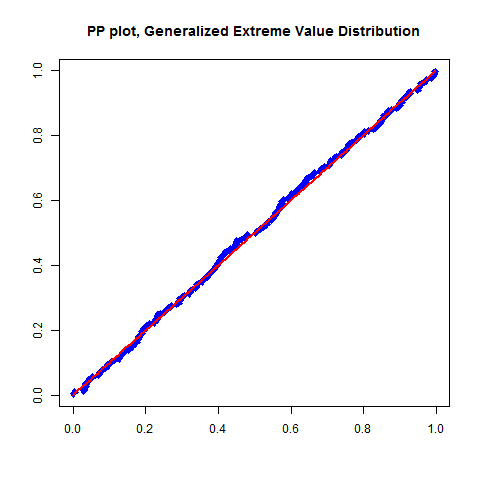
\includegraphics[width=8cm]{SFMTailGEV}
  \caption{PP plot against the Generalized Extreme Value Distribution for portfolio: Bayer, BMW, Siemens. Time period: from 2000-01-01 to 2016-07-11.}
\end{figure}

\end{frame}


	
	
\end{document}
